\documentclass[11pt]{article}
\usepackage[margin=1in]{geometry}
\usepackage{graphicx}
\usepackage{booktabs}
\usepackage{enumitem}
\usepackage{microtype}
\usepackage[hidelinks]{hyperref}
\usepackage{xcolor}
\usepackage{parskip}
\usepackage{caption}
\usepackage{float}
\usepackage{fancyvrb}
\fvset{samepage=true}
\usepackage{tikz}
\usetikzlibrary{arrows.meta,positioning}
\usepackage{tabularx}
\usepackage{placeins}
\usepackage{accsupp}
\usepackage{needspace}
\setlength{\emergencystretch}{1.5em}
\hypersetup{
  pdftitle={Membranes and Portals: A Spatial Interface for cs-mail},
  pdfsubject={Conversation reuse and recipient-defined request classes}
}
\setlength{\parskip}{5pt plus 1pt}

\title{\textbf{Membranes and Portals}\\\large A Spatial Interface for cs-mail}
\author{}
\date{September 2026}

\newcommand{\csmail}{\textit{cs-mail}}
\newcommand{\term}[1]{\textbf{#1}}

% Provisional UI notation: Reference U+2196 (↖), Share U+21F1 (⇱).
% Both glyphs denote interface actions, not protocol syntax.
% Share is drawn as a northwest arrow to a corner; no font or icon asset
% is required. PDF ActualText labels the drawing with its Unicode identity.
\DeclareRobustCommand{\refmark}{\ensuremath{\nwarrow}}
\DeclareRobustCommand{\sharemark}{%
  \BeginAccSupp{method=hex,unicode,ActualText=21F1,space}%
  \tikz[baseline=-0.25ex,x=1ex,y=1ex,
        line width=0.095ex,line cap=butt,line join=miter]{%
    \path[use as bounding box] (0,0) rectangle (1.75,1.75);
    \draw (0.12,0.20) -- (0.12,1.60) -- (1.52,1.60);
    \draw (1.38,0.22) -- (0.40,1.20);
    \draw (0.40,0.67) -- (0.40,1.20) -- (0.93,1.20);
  }%
  \EndAccSupp{}%
}

\begin{document}
\maketitle

\begin{abstract}
Most email interfaces inherit a small collection of objects from conventional electronic mail: inboxes, folders, messages, threads, quoted replies, and compose windows. \csmail{} changes the underlying communication model. It introduces persistent sender--recipient relationships, explicit permission, first-contact requests, constrained express lanes, and a richer distinction between the content used while composing a message and the content actually transmitted. This memo develops two complementary interface concepts for making that structure visible: the \emph{membrane}, which represents access to a user's communication space, and \emph{portals}, which provide spatial navigation through relationships, conversations, messages, and passages. A single conversation-level reuse policy governs Reference, Quotation, and Sharing together, permitting reuse within and across relationships by default or restricting it to the originating relationship. The proposal develops an information architecture and interaction model, including the distinction between private workspace activity and deliberate disclosure.
\end{abstract}

\section{Why a new interface language?}

Most attempts to redesign email retain the ontology of email. They may change prioritization, typography, search, or the arrangement of panes, but the user still moves among an inbox, a thread, an individual message, and a compose window. This is reasonable when the underlying system is itself organized around independently delivered messages and reconstructed threads.

\csmail{} has different native structure. A sender may or may not have standing permission to reach a recipient. A first-contact attempt has a different status from correspondence within an established relationship. A recipient may deliberately create a temporary or purpose-specific route through an otherwise restrictive communication boundary. Relationships persist over time and may contain multiple conversations. Messages and passages can be treated as addressable objects. Each conversation also has a common reuse boundary for referencing, quoting, and sharing its contents.

Rendering all of this as another three-column email client would conceal much of what the protocol changes. The design question is:

\begin{quote}
\emph{What would an interface look like if it were designed around the native objects and semantics of \csmail{}, rather than inherited from conventional email clients?}
\end{quote}

The membrane and portals are one proposed answer.

\Needspace{12\baselineskip}
\section{The membrane: communication has a boundary}

A \term{membrane} is the visible representation of the boundary around a user's communication space. Established, permitted relationships live inside it. First-contact attempts begin outside it. Express lanes form deliberately constructed passages through it.

Recipients can publish up to eight classes of their own at that boundary, with collateral chosen for each within the deployment's collateral bounds. The sender chooses a class and authorizes its fixed terms. These entry points describe invitations to approach; they are not permission grants or permanent kinds of relationship.

The membrane therefore represents protocol state spatially. It is not merely an illustration surrounding an inbox. Its geometry and transitions should correspond to meaningful changes in access:

\begin{itemize}[leftmargin=*]
    \item accepting a request with standing permission opens an ongoing route; accepting with an express lane opens a bounded route, with the full request refund obligation recorded in either case;
    \item revoking that permission closes the future route while preserving the historical correspondence;
    \item a first-contact request can be pulled inward for inspection without thereby granting future access;
    \item an express lane concerns the relationship, potentially limited by identity, purpose, duration, or message density, and is usually not scoped to one conversation.
\end{itemize}

This gives a user a perceptible answer to a question that conventional email clients answer poorly: \emph{who can reach me, and under what conditions?}

The spatial distinction should remain semantically stable. ``Inside'' should indicate authorized communication; a bounded route should remain distinguishable from standing permission. A published request entry point invites an approach without opening either route. Animation is useful when it explains a state transition, such as acceptance opening the route actually granted. It should not exist merely to make the product feel futuristic.

\section{Portals: correspondence is something one moves through}

Conventional email navigation is largely categorical: inbox $\rightarrow$ thread $\rightarrow$ message, followed by back navigation, search, another result, and another thread. The user's current context is repeatedly replaced.

\term{Portals} instead treat correspondence as a nested information space. A useful conceptual hierarchy is:

\begin{center}
\textbf{communication space $\rightarrow$ person $\rightarrow$ conversation $\rightarrow$ message $\rightarrow$ passage.}
\end{center}

Selecting an object need not replace the current screen. It may expand within the current context, open beside it, or temporarily reveal another part of the correspondence space. A person's portal can expand into the history of the relationship. A conversation can unfold into its messages. A message can expand into a reading surface. A reference in a new message can open the older passage to which it points.

``Portal'' is therefore an interaction principle rather than a commitment to a literal glowing circle. The visual language can evolve. The essential property is continuity of context: users should be able to move into relevant correspondence and back out without repeatedly destroying and reconstructing their working arrangement.

\Needspace{10\baselineskip}
\section{The complementary roles of membranes and portals}

The two concepts solve different problems:

\begin{center}
\begin{tabular}{ll}
\toprule
\textbf{Membrane} & Who and what can reach me? \\
\textbf{Portals} & How do I move through and compose with my correspondence? \\
\bottomrule
\end{tabular}
\end{center}

In short, \textbf{membranes represent access; portals represent context}. Their combination gives the interface a visual grammar derived from the protocol itself. Conversation-level reuse indicators add a related distinction: which correspondence may cross into another relationship. That disclosure boundary is separate from permission to contact a person through the membrane.

\section{From threads to structured correspondence}

Traditional email frequently preserves context through textual replication. A reply may contain the previous message, which itself contains an earlier message, producing recursively quoted documents. Email clients then reconstruct those documents into a visual thread.

\csmail{} need not use recursive quotation as its native representation. It can instead treat a relationship as containing conversations, conversations as containing messages, and messages as containing independently addressable passages. Each message contains its own newly transmitted content. Earlier correspondence retains its source identity. A canonical identity does not require a single physical copy or exclude explicitly shared copies.

This suggests a different meaning of ``thread.'' A person may have a durable relationship containing several conversations, such as ``Workshop ideas,'' ``Portfolio feedback,'' and ``Dinner next week.'' Those conversations can be entered through the person's portal rather than appearing only as unrelated rows scattered across an inbox.

The result is a correspondence graph that the portal interface can navigate directly.

\section{Reference without reproduction}

Once previous content is addressable, a new message can \emph{refer} to earlier content without reproducing it. A reference might target an entire earlier message or a particular passage. It may point to material in the current conversation or to material in a previous conversation.

Suppose an earlier message asks, ``Would a single-day event be enough?'' A later message can say, ``I've changed my mind about this. One day is probably enough,'' while carrying a structured reference to the earlier question. The source remains canonical. The later message contains only the new prose.

When the recipient activates the reference, the original passage can open beside the response through a small portal. This replaces a common use of quotation with addressing.

A critical rule follows:

\begin{quote}
\textbf{Reference does not confer access.}
\end{quote}

For a recipient to read the referenced source, that recipient must have access to it. A reference supplies neither an access grant nor source text by itself. A permitted sharing action can explicitly make selected material available when needed. Similarly, placing a message from some other correspondence beside a draft in one's private workspace does not share, forward, or quote it. Disclosure must remain a separate, explicit operation.

This distinction is important because it separates several acts that conventional interfaces can blur: consulting context, transmitting new content, referring to shared context, quoting content, forwarding content, and granting access.

\subsection{A visual language for reference}
\label{sec:reference-language}

The distinction between consulting, referencing, quoting, and sharing needs a visible language. The proposal uses \refmark{} as a compact \term{reference marker} beside the referring sentence or passage, and \sharemark{} as the \term{Share} control. The latter is the northwest-arrow-to-corner glyph (Unicode U+21F1). Both are provisional interface notation, independent of protocol syntax. The reference itself is a structured relation between addressable objects.

\begin{quote}
Reference establishes a connection to existing content. Quotation reproduces content within a new message. Sharing explicitly makes selected content available to specified recipients, through access authorization or delivery. These operations can be combined, but none should silently trigger another.
\end{quote}

\textbf{The operations differ in their effects, while sharing a common conversation-level reuse policy.} Section~\ref{sec:reuse-policy} defines that policy. Separate operation labels do not imply separately configurable permissions.

\begin{table}[htbp]
\centering
\begingroup
\renewcommand{\arraystretch}{1.2}
\small
\begin{tabularx}{\textwidth}{@{}p{0.15\textwidth}p{0.12\textwidth}X@{}}
\toprule
\textbf{Operation} & \textbf{Notation} & \textbf{Meaning} \\
\midrule
Reference & \refmark{} & Points to an existing message or passage. Activating the marker opens the source through a portal; it does not grant access. \\[0.4em]
Quote & ``\ldots'' & Reproduces selected source content in the new message. Sending the message transmits that reproduced content. \\[0.4em]
Share & \sharemark{} & Makes selected material available to specified recipients through access authorization or delivery. Its review shows scope and mechanism; opening the workflow alone discloses nothing. \\
\bottomrule
\end{tabularx}
\endgroup
\caption{Three operations with different effects and one common conversation-level reuse policy. A combined workflow must make each effect explicit.}
\label{tab:reference-notation}
\end{table}

The Share control should carry the text label ``Share'' alongside \sharemark{}. The icon marks an explicit disclosure workflow; \refmark{} marks a navigable connection to context. Neither symbol alone communicates the source conversation's permitted reuse scope, which should be displayed separately.

\paragraph{Naming the parts.}
The \term{source} is the earlier message or passage being referenced. The \term{referring passage} is the part of the new message to which the reference belongs. A \term{passage anchor} identifies the relevant span within a particular message or message version; it should not depend on screen coordinates or line wrapping. A \term{reference connector} is the temporary line shown between the two passages in a workspace. A \term{reference portal} is the source view opened when a reader activates the marker. The portal displays the source, while the reference records how that source relates to the new text.

\paragraph{Creating a reference while composing.}
The author opens earlier correspondence beside a draft, selects a source passage, and chooses ``Reference in draft,'' or uses an equivalent deliberate drag action. The author then associates that source with a sentence or selected passage in the draft. A subtle dotted connector previews the association. Merely opening a message, selecting its text, or moving it beside the draft creates no transmitted reference.

For example, Alex's earlier question, ``Would a single-day event be enough?'' can be associated with the new sentence, ``I think your original instinct was right.'' The source may belong to the current conversation or an older conversation. Both use the same interaction. The author can inspect, change, or remove the association before sending. Removing it leaves the draft's prose and the source unchanged. A proposed outgoing association must satisfy the source conversation's current reuse policy; a connector by itself neither overrides that policy nor grants access.

The connector is a visual relationship between two passages, not copied text. Its on-screen orientation follows the layout; the stored reference points from the referring message or passage to its source regardless of where the two objects are placed.

\paragraph{Collapsing context into a marker.}
When the author closes the source portal, the connector collapses into a compact marker next to the referring passage:

\begin{quote}
I think your original instinct was right.\,\refmark{} Let's keep it to one day.
\end{quote}

The marker means ``this passage has a reference.'' It does not mean ``share,'' ``forward,'' or ``go back.'' Its northwest-pointing shape is a provisional mnemonic for reaching into earlier context; the source need not physically sit above or to the left. The marker is rendered by the client from reference metadata rather than inserted as a literal arrow character into the author's prose.

\paragraph{Reading through the reference.}
Activating \refmark{} opens the source beside the referring passage, highlights the anchored text, and shows its author, date, and conversation where the reader is authorized to see that information. The current message stays visible. The reader can expand the source only to the extent of their authorized access, or close it and continue reading at the same position. Access to a shared passage does not imply access to the containing message, its attachments, or the whole conversation. Closing a portal does not delete its reference.

Figure~\ref{fig:reference-lifecycle} illustrates an allowed reference within the relationship with Alex. The spatial connector, compact marker, and opened source portal are three presentations of that reference.

\begin{figure}[htbp]
\centering
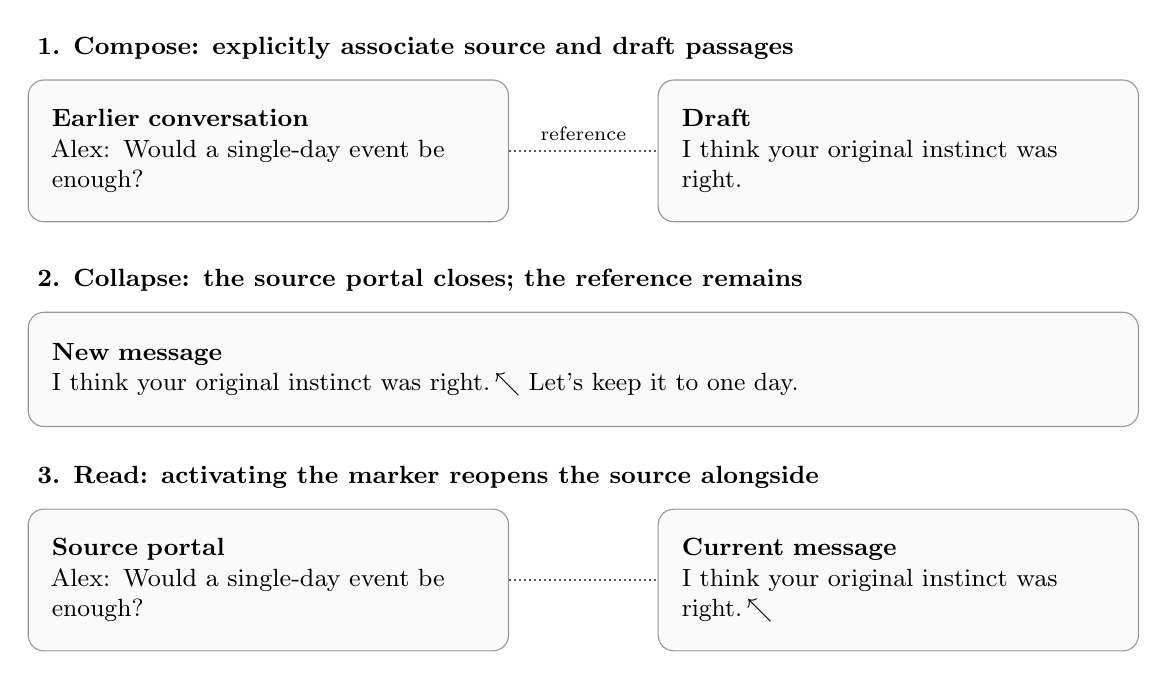
\begin{tikzpicture}[
  x=1cm,y=1cm,
  card/.style={draw=black!40,rounded corners=2mm,fill=black!2,
    text width=5.5cm,inner sep=3mm,align=left,font=\small,
    minimum height=1.8cm,anchor=north west},
  phase/.style={anchor=west,font=\small\bfseries},
  link/.style={densely dotted,line width=0.8pt,draw=black!65}
]
\node[phase] at (0,0.4) {1. Compose: explicitly associate source and draft passages};
\node[card] (source) at (0,0) {\textbf{Earlier conversation}\par
  Alex: Would a single-day event be enough?};
\node[card] (draft) at (8,0) {\textbf{Draft}\par
  I think your original instinct was right.};
\draw[link] (source.east) -- node[above,font=\scriptsize]{reference} (draft.west);

\node[phase] at (0,-2.55) {2. Collapse: the source portal closes; the reference remains};
\node[card,text width=13.5cm,minimum height=1.45cm] at (0,-2.95)
  {\textbf{New message}\par
  I think your original instinct was right.\,\refmark{} Let's keep it to one day.};

\node[phase] at (0,-5.05) {3. Read: activating the marker reopens the source alongside};
\node[card] (opened) at (0,-5.45) {\textbf{Source portal}\par
  Alex: Would a single-day event be enough?};
\node[card] (reading) at (8,-5.45) {\textbf{Current message}\par
  I think your original instinct was right.\,\refmark{}};
\draw[link] (opened.east) -- (reading.west);
\end{tikzpicture}
\caption{An allowed reference within the relationship with Alex, across composition, compact presentation, and reading. The source views are portals onto existing correspondence. Their contents are not automatically included in the new message, and the same conversation-level policy governs quotation and sharing.}
\label{fig:reference-lifecycle}
\end{figure}

\paragraph{Multiple sources and unavailable sources.}
One passage can refer to several sources, and several passages can refer to the same source. A compact count, such as \refmark{}\,2, can indicate two references; activation opens a small source chooser or two portals. The interface should reveal connectors on focus or selection rather than cover the whole message in persistent lines. A reference records an association chosen by its author. It does not by itself certify agreement, support, or the truth of either passage.

Three checks remain distinct. \term{Reuse scope} asks whether the source conversation's current policy permits a new reference into the destination relationship. \term{Access} asks whether the recipient is authorized to read the target. \term{Availability} asks whether the target can actually be retrieved. A permitted reference may still have an unavailable source. The interface should report that state without silently substituting a quotation, widening access, or exposing unauthorized previews or metadata. Before sending, it should check reuse scope and access for the intended recipients and indicate availability where it can be established.

\paragraph{Keeping disclosure explicit.}
The Share icon \sharemark{} opens a review of the exact material, intended recipients, and proposed access change or delivery. The source conversation's current reuse policy determines the permitted relationship scope. An access grant additionally requires authority over the retrieval mechanism; delivering a permitted copy is a different mechanism and must be labeled accordingly. Default permission for cross-relationship reuse does not authorize opening another person's mailbox or all of their correspondence. Nor does access revocation retract a copy already delivered.

Sending a quotation gives its recipients the reproduced text and must satisfy the same conversation-level policy as reference and sharing. Quotation cannot bypass a restriction on the destination relationship. A reference can also reveal information through its target identifier, title, or preview. Review must therefore cover all recipient-visible content and metadata, not just the text exposed when a portal opens.

For example, a message from Sarah may sit beside a draft addressed to Alex for private consultation. Alex gains no access from that arrangement. Creating a reference does not change this. Making Sarah's words available to Alex requires a deliberate disclosure permitted by the source conversation's current policy. The default permits that choice without a fresh reuse-consent request for each recipient; a relationship-only policy rules it out in the ordinary workflow. Drawing a connector makes neither decision.

\paragraph{Legacy recipients and accessible controls.}
The same local reference language can be used when the source originated as conventional email. What the remote reader receives depends on supported capabilities, as discussed in Section~\ref{sec:transport-independence}. A plain \refmark{} character sent to an ordinary email client would not create an operative portal. The sender should instead review a readable external rendering: for example, a selected quotation with attribution, a textual contextual note, or prose without a transmitted reference. Converting a reference into an excerpt is an explicit quotation step subject to the same conversation-level policy. A change of transport or presentation cannot make otherwise restricted reuse eligible.

Every symbolic control needs a readable name and a non-drag equivalent: ``Add reference,'' ``Open reference,'' ``Remove reference,'' ``Quote passage,'' and ``Share.'' Keyboard and screen-reader users should be able to follow the same relationships and return to the same reading or editing position. The semantic distinctions must remain usable without spatial motion, icon recognition, or color.

\FloatBarrier


\section{Conversation-level privacy and reuse}
\label{sec:reuse-policy}

A \term{reuse policy} specifies the relationship scope within which a conversation's contents may be referenced, quoted, or shared. It concerns onward use of correspondence, separately from permission to contact someone through the membrane and authorization to retrieve a particular object.
Request classes do not determine this policy: two research requests involving different correspondents do not share a reuse boundary merely because their labels match.

\begin{quote}
\textbf{Each conversation has a single current reuse policy governing Reference, Quotation, and Sharing together. By default, these operations are permitted within and across relationships. A conversation may instead be restricted to reuse within its originating relationship, including other conversations within that relationship. The current policy applies to all messages in the conversation, regardless of when they were sent.}
\end{quote}

There are no independent policies for individual messages or for the three operations. The user chooses one conversation-level setting.

\subsection{Two settings, one common boundary}

\begin{center}
\begingroup
\small
\renewcommand{\arraystretch}{1.2}
\begin{tabularx}{\textwidth}{@{}p{0.33\textwidth}X@{}}
\toprule
\textbf{Conversation setting} & \textbf{Permitted scope for all three operations} \\
\midrule
Within and across relationships & Reuse in the originating relationship and in other relationships. This is the default. \\[0.5em]
Within this relationship only & Reuse in the originating relationship, including its other conversations. Reuse into a different relationship is restricted. \\
\bottomrule
\end{tabularx}
\endgroup
\end{center}

Default permission for cross-relationship reuse does not publish a conversation, notify anyone, grant retrieval access, or send content. It permits a deliberate action. A reference still supplies no access authority; sharing still requires an explicit choice of content, recipients, and delivery or access mechanism. The common policy determines whether the proposed destination relationship is allowed. Each operation retains its own effects and controls.

\subsection{Conversation scope, relationship boundary}

The \emph{conversation} determines which content is governed. The \emph{originating relationship} determines where restricted content may be reused. In one-to-one correspondence, a relationship with Sarah and a relationship with Alex are distinct even when both people are accepted contacts. Permission does not propagate through a network of acquaintances.

Suppose the user and Sarah have two conversations: ``Unpublished proposal,'' restricted to their relationship, and ``Workshop schedule,'' using the default setting. A passage from the proposal can be referenced or quoted in the scheduling conversation with Sarah. A scheduling message can be deliberately shared with Alex under its conversation's default policy. The proposal cannot be referenced, quoted, or shared into the relationship with Alex while its source conversation is restricted.

The restriction does not make every conversation with Sarah restricted. Conversely, merely displaying, linking, or regrouping the proposal in an unrestricted conversation cannot release it. The source conversation remains identifiable. Provenance is needed to prevent local organization from becoming a bypass; it is not a separate, configurable policy on each message or passage. The treatment of content already reproduced in other conversations is an implementation question identified below.

\subsection{Changes apply to the entire conversation}

When a conversation's policy changes, the permitted reuse of its entire contents changes, including earlier messages. If the user changes ``Unpublished proposal'' to relationship-only, a subsequent attempt to quote an old message from it into a conversation with Alex must obey the current restriction. There is no earlier send-time policy attached to that message. If the conversation is later legitimately returned to the default setting, that current setting likewise governs its entire contents.

The control and confirmation should name the conversation and state the scope of the change. For example: ``Reuse for all messages in Unpublished proposal is now limited to this relationship.'' A draft prepared before the change receives no exemption: its proposed outgoing references, quotations, and shares must be checked again before transmission.

A policy change does not undo a completed disclosure or erase copies already delivered. Whether it also changes an earlier authorization for future remote retrieval is a separate access-management decision. These limits do not create message-specific policy exceptions. They distinguish current rules for subsequent reuse from the consequences of actions that have already occurred.

\subsection{Private context and deliberate disclosure}

Reading, comparing, searching, and arranging one's accessible correspondence remain private workspace activities. A restricted proposal may sit beside a draft to Alex while the user thinks. Neither its presence there nor the user's attention to a passage should be reported to Sarah. Creating a private provisional association is also distinct from transmitting that association as a reference.

The boundary becomes consequential when source content or a reference to it is proposed for an outgoing message. Reference, Quotation, and Sharing undergo the same relationship-scope check. The check covers visible metadata as well as reproduced content: a revealing subject, attribution, or preview must not pass through merely because the recipient cannot open the source. Known derived content produced by the client should retain its source association rather than lose the boundary through a change of wording or format.

If the destination is outside a relationship-only boundary, the ordinary outgoing operation does not proceed. The user can remove the proposed reuse, choose a conversation within the originating relationship, or use a legitimate policy-change process. These choices must be explicit. The client should neither contact the counterparty automatically nor silently replace a blocked reference with a quotation.

\subsection{Enforcement limits and implementation questions}

The intended protection is enforcement of these distinctions in \csmail{}'s native operations and controlled retrieval, together with intelligible disclosure decisions. Readable content can be retained or reproduced independently, so the interface must not promise absolute prevention of redistribution. A reuse setting should not give the sender remote erasure powers over the recipient's records or turn private reading activity into a report to the sender.

Several implementation questions remain separate from the settled model: who may relax a restriction and how participant conflicts are resolved; how clients confirm the current policy before a consequential action; and whether a change withdraws existing retrieval grants. Group relationships also require explicit treatment of audience changes and historical access. Adding a participant must not silently redefine the audience of restricted history.

Content already quoted or delivered into another conversation requires a provenance-aware treatment of subsequent reuse. That treatment must reconcile the source conversation's current boundary with copies that already exist, without turning the design into independent per-message or per-operation policies. This memo records that requirement without selecting a complete inheritance, revocation, or export mechanism.

\section{Composition as a workspace}
\label{sec:composition}

The portal model changes composition itself. A conventional compose window is primarily a blank document, perhaps with a quoted history beneath it. A portal-based composer can instead be a temporary working arrangement of correspondence.

A user might pull two messages beside one another and write between them. The two messages may be from the same conversation, from different conversations with the same person, or, for private consultation, from entirely different parts of the user's correspondence. The user might compare two proposals, answer several questions, or consult an old exchange while composing a new response.

The crucial principle is:

\begin{quote}
\textbf{Context used to write a message is not necessarily context transmitted with the message.}
\end{quote}

The spatial arrangement is private workspace state, whether temporary or saved as part of a draft. Nothing is forwarded or shared merely because it has been brought into the composition surface. When the source conversation's current reuse policy permits the destination relationship, the author may explicitly associate a draft passage with the source. Recipient access remains a separate check; where additional disclosure is permitted and needed, a deliberate sharing action can accompany the reference.

A persistent source-portal indicator can read \textbf{Reuse: Within this relationship only}, with the originating relationship named nearby. The destination composer separately identifies its recipients. Opening Sarah's restricted proposal beside a draft to Alex is permitted private consultation, while the differing relationship labels explain why its content cannot be included in that outgoing message.

The same boundary applies whether the author chooses \refmark{}, inserts a quotation, or uses \sharemark{}. A provisional connector should show an unresolved or restricted state rather than resemble a completed, sendable reference. Checks are repeated when recipients change, when the conversation policy changes, and before sending. A mismatch should identify the source conversation and offer explicit choices without transmitting any source material.

This makes composition a workspace for thinking with correspondence while retaining a visible distinction between the context being consulted and the context being sent.

\section{Transport Independence and Legacy Correspondence}
\label{sec:transport-independence}

The membrane and portal concepts should apply to correspondence regardless of the transport by which a message arrived. This is especially important during adoption: a \csmail{} user may have regular correspondence with people who continue to use Gmail or another conventional email provider. Relegating those correspondents to a separate legacy interface would reproduce a provider boundary that is irrelevant to the user's actual relationships.

The governing principle is:

\begin{quote}
\textbf{The correspondence model presented to the user should not be determined by the transport mechanism through which a message arrived.}
\end{quote}

Transport remains important as provenance and for determining which protocol capabilities are available. It need not determine the primary information architecture.

\subsection*{Correspondence is not transport}

Conventional email clients largely expose transport-native objects directly: RFC/MIME messages are grouped into folders and inferred threads, and replies often carry copied fragments of earlier messages. \csmail{} can separate the transport layer from the correspondence layer:

\begin{Verbatim}[fontsize=\small]
Transport layer                 Correspondence layer

SMTP message ---------+              Relationship
                      +---------->        |
cs-mail message -------+              Conversation
                                          |
                                       Message
                                          |
                                       Passage
\end{Verbatim}

An SMTP message is therefore input to the \csmail{} correspondence model rather than an instruction to reproduce the presentation conventions of an SMTP client. A useful shorthand is:

\begin{quote}
\textbf{Transport is provenance. Correspondence is the interface.}
\end{quote}

The transport origin should remain inspectable when relevant, but it should normally occupy the role of metadata rather than navigation.

\subsection*{Normalizing legacy email into native correspondence}

When a conventional message enters \csmail{}, the original RFC/MIME object should be preserved. A normalized representation can then be constructed for ordinary interaction. Conceptually, ingestion proceeds as follows:

\begin{Verbatim}[fontsize=\small]
RFC/MIME message
      |
preserve original
      |
parse structure
      |
identify sender-recipient relationship
      |
recover reply/reference relationships
      |
separate novel content from quoted history
      |
normalize attachments and metadata
      |
cs-mail correspondence object
\end{Verbatim}

Preservation of the original is important. Normalization is a view over the evidence, not destructive conversion. The user should be able to inspect the original message when parsing, signatures, unusual MIME structure, or other transport details matter.

This permits \csmail{} to suppress much of the textual redundancy of conventional replies. For example, an incoming Gmail message might contain:

\begin{Verbatim}[fontsize=\small]
Sounds good. Thursday works.

On Tuesday Marcus wrote:
> Thursday or Friday works.
>
> On Monday Alex wrote:
>> What day should we meet?
\end{Verbatim}

If the quoted material corresponds to messages already present in the local correspondence history, the native view can instead render:

\begin{Verbatim}[fontsize=\small]
Alex
    What day should we meet?

Marcus
    Thursday or Friday works.

Alex
    Sounds good. Thursday works.
\end{Verbatim}

The legacy message has thereby become usable as a native \csmail{} object without pretending that its transport origin was something other than SMTP.

\subsection*{A unified membrane}

The membrane should represent permission rather than provider membership. An accepted Gmail identity can therefore occupy the same interior communication space as a native \csmail{} identity:

\begin{Verbatim}[fontsize=\small]
                         REQUESTS

      Unknown Gmail sender o

                 +------------------+
                 |                  |
                 |   o Alex         |
                 |     Gmail        |
                 |                  |
                 |         o Sarah  |
                 |           cs-mail|
                 |                  |
                 +------------------+
\end{Verbatim}

The provider or transport may be shown subtly where useful, but it is not the primary spatial distinction. A previously accepted external correspondent is inside the membrane because a communication relationship exists. An unknown native \csmail{} sender can still begin outside it.

This strengthens the membrane metaphor. The boundary is social and protocol-level: it expresses routes of permitted communication, not membership in a particular service.

\subsection*{Portals over legacy correspondence}

The same transport independence should extend to portals. A Gmail correspondent can have a person portal, conversations, messages, passages, and a navigable history just like a native \csmail{} correspondent. Imported SMTP messages can participate in spatial composition as ordinary correspondence objects.

For example, while writing a new message to Alex, the user might open an old Gmail-originating message beside the draft:

\begin{Verbatim}[fontsize=\small]
OLD GMAIL MESSAGE                 DRAFT

+--------------------+       +-----------------------+
| Alex - April 12    |       |                       |
|                    |       | I think your          |
| Would a single-day |......>| original instinct     |
| event be enough?   |       | was right.            |
+--------------------+       +-----------------------+
\end{Verbatim}

From the author's perspective, there is no reason for this operation to feel different merely because the left-hand object originally arrived as MIME over SMTP. The portal operates over correspondence, not over transport protocols.

This is particularly useful for long-running relationships. A user should be able to experience years of correspondence through the same spatial system even if the counterparty has never created a \csmail{} account.

\subsection*{Asymmetric capabilities and graceful degradation}

A unified interface must not imply that all transports possess the same semantics. It is therefore useful to distinguish \emph{local} capabilities from \emph{bilateral} capabilities.

Local capabilities can be provided by the \csmail{} client even when the counterparty uses conventional email. These include membrane organization, person portals, locally inferred conversation structure, suppression of recognized redundant quotation, side-by-side historical context, and spatial composition.

Other capabilities require native support at both ends. Protocol-native passage references are a clear example. If two \csmail{} users communicate, a new message can contain a structured pointer to an earlier message or passage. A conventional Gmail client does not understand that primitive.

The appropriate response is graceful serialization. A native relation such as

\begin{Verbatim}[fontsize=\small]
Message 73
    |
    +-- refers-to --> Message 12, passage 4
\end{Verbatim}

can, where context is needed, be represented externally as ordinary readable email, for example:

\begin{Verbatim}[fontsize=\small]
I think your original instinct was right.

Regarding your April 12 question:
"Would a single-day event be enough?"
\end{Verbatim}

The precise external rendering remains a design question. A sender may choose a quoted excerpt, a conventional reply header, or prose without a transmitted reference. Every choice that transmits source content or reference metadata must satisfy the source conversation's current reuse policy. A permitted native operation may become intelligible conventional communication; serialization cannot grant permission that the native operation lacked.

For example, a relationship-only passage from an older conversation with Alex can be quoted in a new email to Alex within that relationship. It cannot be sent to Sarah merely because the client converts a reference into plain text. The same scope applies to Reference, Quotation, and Sharing. Material consulted privately is not disclosed by the transport adapter, and an outgoing preview should show exactly what is being transmitted.

\subsection*{Reuse policy at the legacy boundary}

Imported conventional correspondence may have no recorded \csmail{} reuse policy. The interface should distinguish a local default or user-applied restriction from a policy communicated or agreed through the native protocol. It may show ``No native policy recorded'' alongside the locally applied setting; it must not attribute an affirmative grant or agreement to an external sender without evidence.

A local policy can govern the \csmail{} client's actions. It does not imply matching controls in a Gmail recipient's client. Sending a quotation, shared passage, or attachment over ordinary email delivers the selected material outside native enforcement. The sender should see that consequence before transmission. A controlled-access portal could offer a different delivery mechanism, but readable content remains independently reproducible. Access enforcement and the common relationship-scope policy should remain distinguishable.

Transport-origin metadata, import grouping, and later regrouping must not silently release a known restriction. Recovering conversations from legacy mail and recognizing independently received duplicates require explicit provenance and identity handling; a new visual grouping alone should not be treated as a new privacy decision.

\subsection*{Progressive enrichment}

Transport independence suggests a useful model of adoption. Consider a relationship in three stages:

\begin{Verbatim}[fontsize=\small]
Stage 1
Marcus: cs-mail        Alex: Gmail
Native cs-mail UX locally; SMTP interoperability remotely.

Stage 2
Marcus: cs-mail        Alex: Gmail plus a cs-mail identity
Some bilateral native capabilities become available.

Stage 3
Marcus: cs-mail        Alex: cs-mail
Full native correspondence semantics are available.
\end{Verbatim}

The relationship should not have to be recreated as these capabilities change. If Alex's Gmail identity has already been associated with the relationship, later adoption can enrich the existing object with additional identities and protocol capabilities.

Thus \csmail{} adoption can be understood as \emph{capability enrichment rather than migration between communication universes}. The user's social world remains continuous while the semantics available within particular relationships become richer.

\subsection*{Bootstrapping the cs-mail experience from existing correspondence}

This architecture has an important product consequence. A new user need not begin with an empty membrane and wait for other people to join. Existing conventional correspondence can be imported and organized immediately.

Rather than presenting migration primarily as a count of imported messages, \csmail{} can reconstruct the user's correspondence space:

\begin{Verbatim}[fontsize=\small]
                 YOUR CORRESPONDENCE

             +-----------------------+
             |                       |
             |  o Alex               |
             |  o Nina               |
             |  o Marta              |
             |  o Russell            |
             |  o Family             |
             |                       |
             +-----------------------+

              327 inferred relationships
               41 need your review
\end{Verbatim}

Much of this reconstruction can rely on deterministic and inspectable evidence: participants, Message-ID and References headers, bidirectional communication history, reply behavior, recency, frequency, address-book membership, and mailing-list or bulk-message indicators. Ambiguous cases can be surfaced for user review rather than silently asserted. Automated inference may assist, but the core migration should remain explainable, reversible, and correctable.

The result is that a user can experience the central \csmail{} interface on the first day. Existing relationships inhabit the membrane. Their histories become portals. Old messages can participate in spatial composition. As counterparties later adopt native \csmail{}, those same relationships progressively acquire structured references, richer permission semantics, express lanes, and other bilateral capabilities.

Interoperability is therefore better understood as an \emph{ingestion boundary} than as a compatibility screen at the edge of the product. Once correspondence crosses that boundary, \csmail{} can represent it according to its own information architecture while preserving the original transport evidence and respecting the capabilities of the remote system. This materially changes the adoption problem: the value of the interface need not wait for network-wide migration.

\section{Worked example}

Consider an established correspondent, Alex. Because Alex has standing permission, Alex is represented inside the user's membrane. Alex sends a message concerning a fall workshop. The earlier conversation containing the original proposal is set to \emph{Within this relationship only}.

The user enters Alex's portal. The relationship contains several conversations, including an older ``Workshop proposal'' conversation and the current ``Fall workshop'' conversation. While composing a response, the user remembers that Alex previously raised a question about whether the event should last one or two days.

Rather than leaving the composer, searching, opening another thread, copying text, returning, and pasting it, the user opens the older conversation beside the draft. The relevant old message becomes one object in the current workspace; the current message becomes another. The draft sits between them.

The user writes: ``I think your original instinct was right.\,\refmark{} Let's keep it to one day.'' The first sentence is associated with Alex's earlier question through an explicit reference action. Closing the older portal leaves the draft and its compact \refmark{} marker in place, following the lifecycle described in Section~\ref{sec:reference-language}.

This use is permitted: the source and destination conversations both belong to the relationship with Alex. The restriction is relationship-scoped rather than limited to the original conversation. When the message is sent, Alex receives the new prose and a reference to correspondence Alex already possesses. Activating \refmark{} opens the old question beside the new answer. No recursively quoted copy of the old message is necessary.

Now the user opens the same proposal beside a draft to Sarah. Private consultation remains available. A proposed outgoing reference to it, quotation from it, or share of it is restricted by the same source-conversation setting. The interface identifies the relationship mismatch; changing the presentation from a portal to copied text does not resolve it.

If the proposal conversation instead has the default setting, deliberate reuse into the relationship with Sarah is permitted. A review can offer ``Share the selected passage with Sarah and add a reference.'' The user sees the selected text, accompanying metadata, intended recipient, and delivery mechanism. Sarah receives only that approved selection; the reference opens it without exposing the remaining proposal or the user's other correspondence with Alex.

Changing the proposal conversation's policy while either draft is open updates the decision for all its source messages, including old ones. The check consults the conversation's current setting. It does not attach a separate policy to the draft's selected passage.

The example combines the central principles: portals bring context into thinking and writing, the conversation supplies one current policy for all three operations, and deliberate disclosure remains separate from spatial proximity.

\section{Utility}

The proposal is useful only if its spatial novelty produces concrete advantages. Several follow directly from the model.

\subsection*{Comprehension}
Access relationships become visible rather than buried in settings and filtering rules. The membrane provides a persistent representation of whether a route into the user's communication space exists and what kind of route it is.

\subsection*{Context preservation}
Portals allow users to inspect older correspondence without repeatedly abandoning their present task. Long histories can be traversed while maintaining a stable working context.

\subsection*{Composition}
Messages and passages become material that can be temporarily arranged around a draft. The user can compare, consult, and respond to several pieces of correspondence simultaneously.

\subsection*{Less textual redundancy}
Structured references can replace many uses of recursive quotation. Historical messages remain canonical objects rather than being reproduced inside every subsequent message.

\subsection*{Privacy and intentional disclosure}
The model distinguishes private workspace context from transmitted content. Arranging something near a draft does not disclose it. Referring to something does not grant access. One current policy per source conversation governs the relationship scope of Reference, Quotation, and Sharing, for all its messages. A visible relationship-only boundary can prevent unintended cross-relationship reuse while leaving private consultation and reuse in other conversations within the originating relationship available.

\subsection*{Correspondence as durable structure}
At its most ambitious, the model treats correspondence as structured, navigable knowledge rather than as a pile of documents. Relationships, conversations, messages, passages, and references retain their identity over time and can be revisited directly.

\section{Design constraints}

The membrane and portal metaphors should impose discipline rather than license arbitrary visual effects.

\begin{itemize}[leftmargin=*]
    \item \textbf{Spatial meaning must be stable.} Inside, outside, passages, and references should have consistent meanings.
    \item \textbf{Motion should communicate state change.} Animation should explain where an object came from, where it went, or what relationship changed.
    \item \textbf{Reading should remain conventional.} Once a user is reading or writing prose, legibility and familiar text interaction take priority over spatial novelty.
    \item \textbf{Spatial manipulation must not imply disclosure.} Workspace arrangement is private unless the user explicitly performs a transmitting or sharing action.
    \item \textbf{Consequential actions must remain explicit.} Selecting a request class, inspecting a request, and granting standing or lane permission are distinct actions. Permission, disclosure, and policy changes must not occur as accidental side effects of exploratory gestures.
    \item \textbf{One policy governs the whole conversation.} Reference, Quotation, and Sharing use the same current setting for all messages. Policy controls must name the conversation and must not imply a selected-message exception or independent operation toggles.
    \item \textbf{Source identity must survive local organization.} Moving a portal, regrouping messages, or changing a transport rendering must not release the source conversation's restriction. Reproduction and already-delivered copies need an explicit provenance model.
    \item \textbf{Recipient agency and enforcement limits remain visible.} Private reading and workspace activity should not notify counterparties. A reuse restriction does not erase existing records or guarantee that readable content cannot be retained independently.
    \item \textbf{Accessible equivalents are required.} Keyboard navigation, screen readers, reduced-motion modes, and non-drag alternatives must expose the same semantics.
    \item \textbf{The metaphor must degrade gracefully.} A user should not need to learn the terms ``membrane'' and ``portal'' in order to operate the client.
\end{itemize}

\section{Implementation note}

The interaction model does not inherently require a game engine. A desktop \csmail{} client can plausibly implement the ordinary reading and composition surfaces with standard HTML/CSS UI, while an SVG or similar vector layer renders membrane geometry, connections, clipping, and transitions. Portal expansion can be expressed as interpolation between spatial layouts while ordinary text controls remain conventional interface elements. More advanced GPU rendering can remain an optimization for effects that later prove difficult to achieve performantly; it need not define the initial architecture.

Request classes, atomic lane acceptance, and native lane-based delivery are implemented in the headless libraries. A separate lane-management grant also resolves a pending request; future access follows the lane without a new bond. Conversation reuse policy remains separate from contact permission.

This separation is desirable in its own right. The spatial layer communicates relationships and state, while the ordinary UI layer preserves mature browser behavior for text selection, editing, accessibility, keyboard navigation, and responsive layout.

The reuse policy belongs to the conversation object. An outgoing Reference, Quotation, or Sharing operation consults that source conversation's current setting and the destination relationship, alongside separate access and availability checks. A passage anchor identifies source content; it carries no independent user-configurable policy or send-time policy snapshot. Source provenance and any record of earlier disclosures serve different purposes from the current policy itself.

Policy checks should be shared by native UI actions and legacy serialization rather than implemented only as a visual warning on one button. Synchronization, race handling, and disconnected operation need a defined method of confirming the current conversation state. Where that state cannot be established, the interface should expose the uncertainty before a consequential action rather than imply that an old local setting is authoritative.

\section{Conclusion}

Membranes and portals give \csmail{}'s underlying structure a visible form.

The membrane makes access perceptible. Portals make context navigable. Structured references allow earlier correspondence to retain its identity while participating directly in later communication. One current conversation-level policy governs Reference, Quotation, and Sharing together: across relationships by default, or within the originating relationship when restricted. The composition workspace lets users arrange the context they need to think while keeping policy, access, and deliberate disclosure distinct.

If \csmail{} changes the structure of electronic correspondence, its interface should make that change intelligible.

\clearpage
\appendix
\section{Concept Mockups}

The following mockups were generated during the design exploration. They are illustrative rather than prescriptive: typography, colors, geometry, and controls may change. They predate the conversation-level reuse policy and request classes, so omit their indicators and the two acceptance choices. The current prose governs those refinements; these historical images are retained unchanged.

\begin{figure}[H]
    \centering
    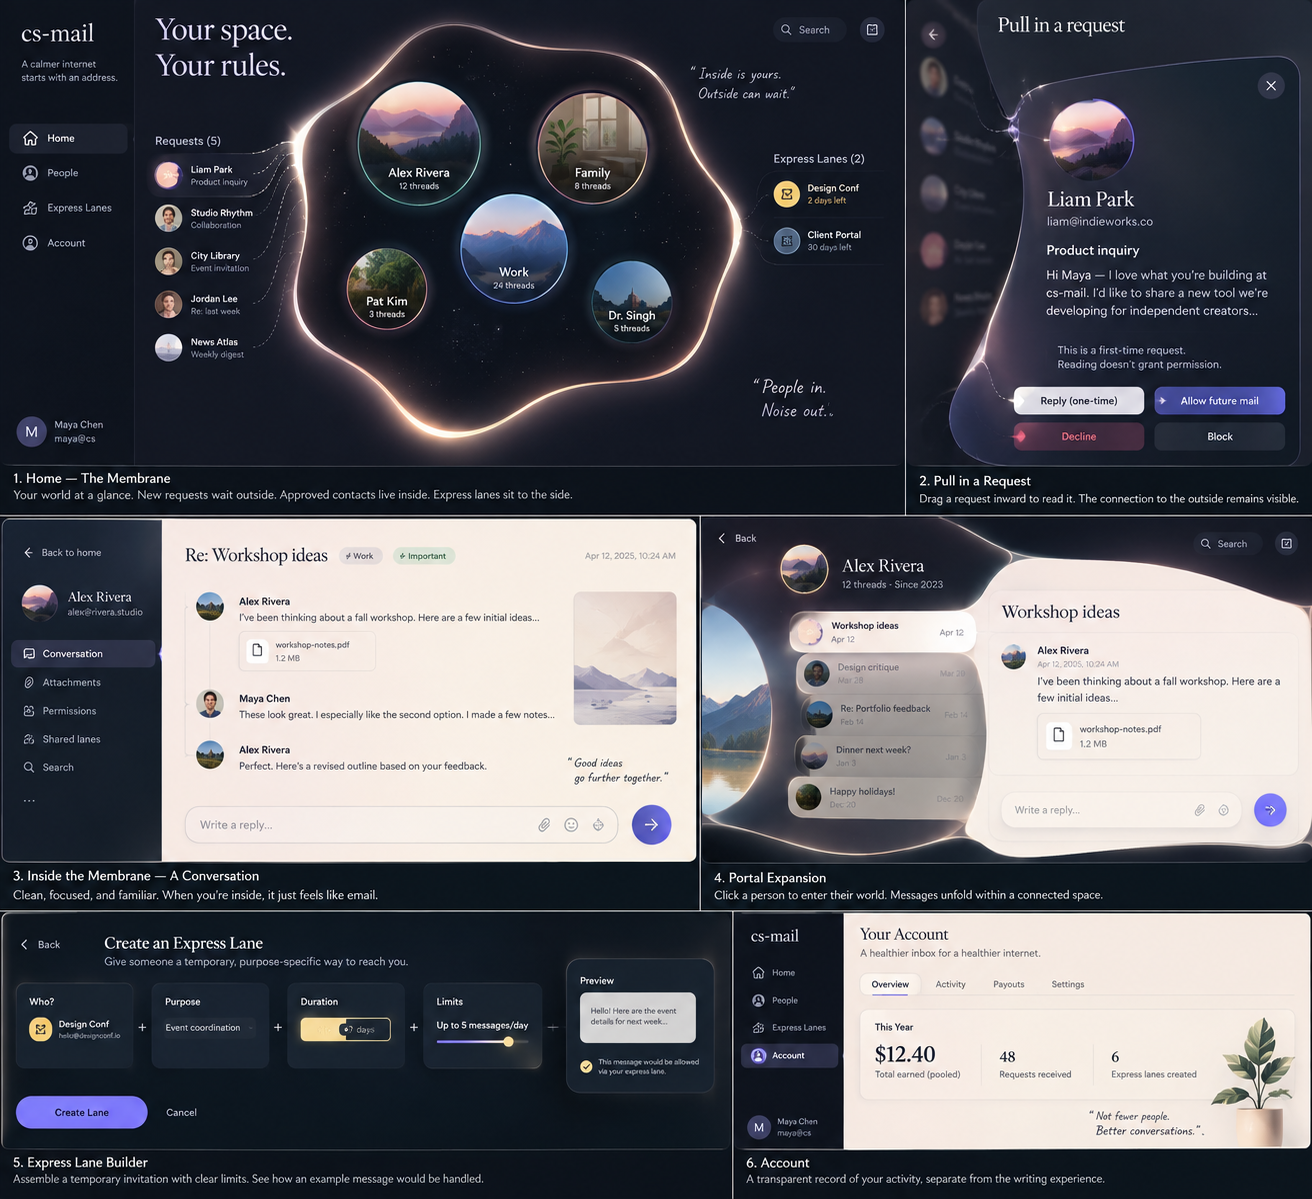
\includegraphics[width=\textwidth]{a_wide_high_resolution_ui_concept_collage_with_a.png}
    \caption{Initial membrane and portals exploration. The panels illustrate the communication membrane, pulling a first-contact request inward for inspection, an ordinary conversation inside the membrane, portal expansion into a correspondent's space, an express-lane builder, and an account view.}
    \label{fig:membrane-portals}
\end{figure}

\clearpage
\begin{figure}[H]
    \centering
    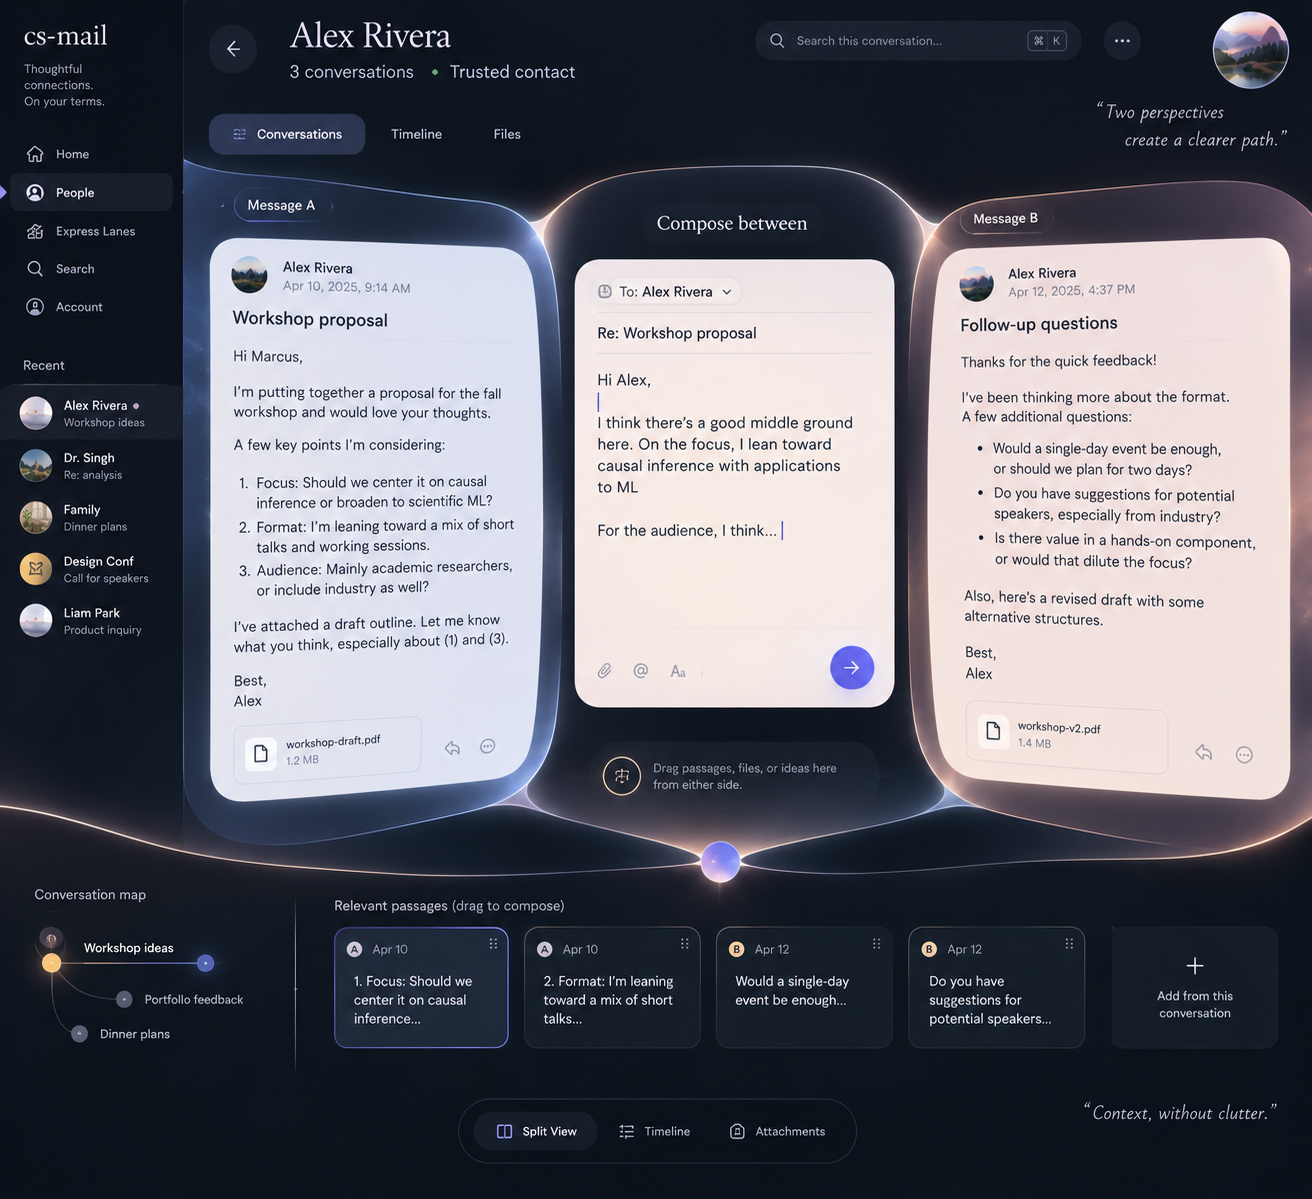
\includegraphics[width=\textwidth]{a_polished_futuristic_ui_concept_illustration_ci.png}
    \caption{Spatial composition exploration. Two earlier messages are opened beside a draft so that the author can consult both while writing. The lower ``relevant passages'' and conversation-map elements shown here were subsequently judged unnecessary; the preferred design acts directly on passages in the opened messages, allowing explicit references to be created without a separate relevance tray.}
    \label{fig:spatial-compose}
\end{figure}

\end{document}
